\documentclass[11pt,a4paper]{article}
\usepackage[T1]{fontenc}
% Packages
\usepackage[margin=1in]{geometry}
\usepackage{amsmath, amssymb, amsthm}
\usepackage{dsfont}
\usepackage{graphicx}
\usepackage{hyperref}
\usepackage{listings}
\usepackage{xcolor}
\usepackage{tikz}
\usepackage{algorithm}
\usepackage{algpseudocode}
\usepackage{booktabs}
\usepackage{enumitem}
\usepackage{array}
\usepackage{float}

% Theorem Environments
\theoremstyle{definition}
\newtheorem{definition}{Definition}[section]
\theoremstyle{plain}
\newtheorem{theorem}{Theorem}[section]
\newtheorem{lemma}[theorem]{Lemma}
\newtheorem{corollary}[theorem]{Corollary}
\theoremstyle{remark}
\newtheorem*{remark}{Remark}

% Listings Configuration
\lstset{
    basicstyle=\ttfamily\small,
    keywordstyle=\color{blue},
    commentstyle=\color{gray},
    stringstyle=\color{green!60!black},
    showstringspaces=false,
    breaklines=true,
    frame=single,
    captionpos=b,
}

% Document Information
\title{Resurse examen SD}
\author{Seria 15}
\date{\today}

\begin{document}

\maketitle
\tableofcontents
\newpage

\section{Sortări}
Algoritmii de sortare pot fi clasificați după complexitate, spațiu, stabilitate și dacă se bazează pe comparații:

\subsection{Clasificare}
\begin{itemize}
  \item \textbf{Elementari:} Insertion, Selection, Bubble
  \item \textbf{Divide et Impera:} Merge Sort, Quick Sort
  \item \textbf{Heap-based:} Heap Sort
  \item \textbf{Non-comparative:} Counting Sort, Radix Sort, Bucket Sort
\end{itemize}

\subsection{Stabilitate}
Un algoritm de sortare este \emph{stabil} dacă menține ordinea relativă a elementelor egale. Acest lucru este important când sortăm obiecte cu multiple chei.

\subsection{Tabel de complexități}
\begin{table}[h]
  \centering
  \begin{tabular}{l c c c c}
    \toprule
    \textbf{Algorithm}
      & \multicolumn{3}{c}{\textbf{Time Complexity}}
      & \textbf{Space (worst)} \\
    \cmidrule(lr){2-4}
      & \textbf{Best} & \textbf{Average} & \textbf{Worst} & \\
    \midrule
    Quicksort     & $\Omega(n\log n)$ & $\Theta(n\log n)$ & $O(n^2)$      & $O(\log n)$     \\
    Mergesort     & $\Omega(n\log n)$ & $\Theta(n\log n)$ & $O(n\log n)$  & $O(n)$          \\
    Timsort       & $\Omega(n)$       & $\Theta(n\log n)$ & $O(n\log n)$  & $O(n)$          \\
    Heapsort      & $\Omega(n\log n)$ & $\Theta(n\log n)$ & $O(n\log n)$  & $O(1)$          \\
    Bubble Sort   & $\Omega(n)$       & $\Theta(n^2)$     & $O(n^2)$      & $O(1)$          \\
    Insertion Sort& $\Omega(n)$       & $\Theta(n^2)$     & $O(n^2)$      & $O(1)$          \\
    Selection Sort& $\Omega(n^2)$     & $\Theta(n^2)$     & $O(n^2)$      & $O(1)$          \\
    Tree Sort     & $\Omega(n\log n)$ & $\Theta(n\log n)$ & $O(n^2)$      & $O(n)$          \\
    Shell Sort    & $\Omega(n\log n)$ & $\Theta\bigl(n(\log n)^2\bigr)$ & $O\bigl((n\log n)^2\bigr)$ & $O(1)$ \\
    Bucket Sort   & $\Omega(n + k)$   & $\Theta(n + k)$   & $O(n^2)$      & $O(n + k)$      \\
    Radix Sort    & $\Omega(n\,k)$    & $\Theta(n\,k)$    & $O(n\,k)$     & $O(n + k)$      \\
    Counting Sort & $\Omega(n + k)$   & $\Theta(n + k)$   & $O(n + k)$    & $O(n + k)$      \\
    Cubesort      & $\Omega(n)$       & $\Theta(n\log n)$ & $O(n\log n)$  & $O(n)$          \\
    \bottomrule
  \end{tabular}
  \caption{Array Sorting Algorithms: time and space complexities}
  \label{tab:sorting}
\end{table}


\subsection{Informații generale}
\begin{itemize}
  \item Sortările prin comparație au limită inferioară $\Omega(n\log n)$.
  \item Algoritmii non-comparativi (Counting, Radix) pot ajunge la $O(n)$ în condiții favorabile.
  \item Alegerea pivotului în Quick Sort influențează performanța:
  \begin{itemize}
    \item pivot ales random
    \item mediana din 3/5/7
    \item mediana medianelor
  \end{itemize}
  \item Pentru vectori mici, sortarea cu algoritmi $O(n^2)$ poate fi mai eficientă decât în $O(n\log n)$ (constanta poate fi mare).
\end{itemize}

\subsection{Counting sort}
Se creează un vector de frecvență cu valorile pe care trebuie să le sortăm. Valorile din vector sunt numărate, iar vectorul este reconstruit în ordine
sortată prin parcurgerea vectorului de frecvență.\\

\noindent
Se aplică când elementele sunt numere întregi într‐un interval \([0, k]\), (până la $10^6$)

\subsection{Bucket sort}
Se creează $k$ buckets și fiecare element $x$ din vectorul de intrare este distribuit în găleata indexată de o funcție de mapare (de ex.\ $\lfloor k\cdot\frac{x-a}{b-a}\rfloor$ pentru valori în $[a,b]$). Fiecare găleată este sortată intern (adesea prin Insertion Sort), apoi se concatenează conținutul găleților pentru a obține vectorul sortat.\\

\subsection{Radix sort}
Sortarea se face pe mai multe trepte de cifre: pentru fiecare poziție de cifră (de la LSD la MSD sau invers) se aplică Counting Sort pentru a grupa elementele după valoarea cifrei curente. După procesarea tuturor cifrelor, vectorul devine complet sortat.\\

\subsection{Quicksort}
Algoritmul Quick Sort folosește o abordare divide et impera: se selectează un pivot, iar vectorul este repartizat în două subsecțiuni, una cu elemente mai mici și cealaltă cu elemente mai mari decât pivotul. Se aplică recursiv același procedeu pe cele două subsecțiuni și, ulterior, se combină rezultatele pentru a obține vectorul sortat.\\

\subsection{Mergesort}
Merge Sort divide recursiv vectorul în jumătăți până se obțin secvențe cu un singur element (sau 2, depinde de implementare). Apoi, aceste secvențe sunt interclasate (merge) după ce au fost sortate, fiind combinate treptat pentru a forma vectorul sortat final.\\

\section{Complexități}

În studiul algoritmilor, folosim trei noțiuni fundamentale pentru a măsura creşterea funcţiei de timp \(T(n)\) în raport cu dimensiunea de intrare \(n\):

\begin{itemize}
  \item \(\mathbf{O}\) (Big-O): reprezintă o limită superioară asimptotică.
    \[
      T(n) = O(f(n)) \iff \exists\, c>0,\; n_0:\;\forall n\ge n_0,\; T(n)\le c\,f(n).
    \]
  \item \(\boldsymbol{\Omega}\) (Big-Omega): reprezintă o limită inferioară asimptotică.
    \[
      T(n) = \Omega(f(n)) \iff \exists\, c>0,\; n_0:\;\forall n\ge n_0,\; T(n)\ge c\,f(n).
    \]
  \item \(\boldsymbol{\Theta}\) (Big-Theta): când există simultan limite superioară și inferioară de același ordin.
    \[
      T(n) = \Theta(f(n)) \iff T(n) = O(f(n)) \;\wedge\; T(n) = \Omega(f(n)).
    \]
\end{itemize}

\noindent
Astfel, \(\Theta(f(n))\) indică creşterea „exactă” (în sens asimptotic), iar $O$ şi $\Omega$ doar conturul superior, respectiv inferior.

% \section{Hash-uri și Tabele de Dispersie}
% Secțiune complexă și completă în LaTeX pentru cursurile de Structuri de Date
\section{Hash-uri și Tabele de Dispersie}
\label{sec:hashuri}

\subsection{Definiții și noțiuni introductive}
\begin{definition}[Funcție de hash]
O \emph{funcție de hash} este o funcție matematică
$$h: \mathcal{U} \to \{0,1,\dots,m-1\},$$
care transformă orice element din universul de chei $\mathcal{U}$ într-o valoare de dimensiune fixă. Rezultatul $h(x)$ se numește \emph{cod hash} al lui $x$. Funcția trebuie să fie eficient de calculat și să distribuie uniform cheile.
\end{definition}

\begin{itemize}
  \item \textbf{Hash prin diviziune:} $h(x) = x \bmod p$, unde $p$ este un număr prim apropiat de $m$.
  \item \textbf{Hash prin multiplicare:} Hash-ul prin multiplicare standard folosește formula
\[
  h_a(K) = \left\lfloor \frac{(aK \bmod W)}{W/M} \right\rfloor,
\]
care produce o valoare în \(\{0,\dots,M-1\}\). Parametrul \(a\) se alege coprim cu \(W\) și cu o reprezentare binară „aleatorie” a biților. În cazul special când \(W = 2^w\) și \(M = 2^m\), formula devine
\[
  h_a(K) = \left\lfloor \frac{(aK \bmod 2^w)}{2^{\,w-m}} \right\rfloor,
\]
  \item \textbf{Proprietate dorită:}\hspace{1em} ipoteza dispersiei uniforme simple, adică pentru orice chei distincte $x,y$ avem
  $$\Pr[h(x)=h(y)] = \frac{1}{m}.$$
\end{itemize}

\subsection{Tabelă cu adresare directă}
\label{subsec:adresare-directa}
Pentru $N$ chei dintr-un univers mic $\{1,\dots,N\}$, putem implementa direct o tăblă de dispersie printr-un vector binar:
\[
  A[1\dots N], \quad A[i] = \begin{cases}1 & \text{dacă }i\text{ este prezent,} \\ 0 & \text{altfel.}\end{cases}
\]
Operații:
\begin{itemize}
  \item \texttt{insert(x)}: $A[x] \leftarrow 1$, cost $O(1)$.
  \item \texttt{find(x)}: returnează $A[x]$, cost $O(1)$.
  \item \texttt{delete(x)}: $A[x] \leftarrow 0$, cost $O(1)$.
\end{itemize}

\subsection{Tabele de dispersie cu coliziuni}
\label{subsec:coliziuni}
Pentru universuri mai mari sau chei arbitrare, folosim o funcție de hash $h$ și rezolvăm coliziunile prin:
\begin{enumerate}
  \item \textbf{Listă înlănțuită (chaining).}
  \item \textbf{Adresare deschisă (open addressing).}
\end{enumerate}

\subsubsection{Chaining}
Fie $T[0\dots m-1]$ un vector de liste înlănțuite. La inserare, adăugăm $x$ în lista $T[h(x)]$. Căutarea parcurge lista, cost amortizat $O(1 + \alpha)$, unde $\alpha = n/m$.

\subsubsection{Adresare deschisă}
Coliziunile se rezolvă prin sondaj:\\
\begin{description}
  \item[Lineară:] $h(x,i) = (h_0(x) + i) \bmod m$.
  \item[Dublu hashing:] $h(x,i) = (h_1(x) + i\cdot h_2(x)) \bmod m$.
\end{description}
În cel mai rău caz, operațiile costă $O(m)$, dar dacă $\alpha < 1$ și funcțiile sunt bine alese, costul mediu este $O(1)$.

\subsection{Dispersie universală}
\label{subsec:dispersie-universala}
\begin{definition}[Familie universală]
O familie de funcții de dispersie $\mathcal{H}$ este \emph{universală} dacă pentru orice $x\neq y$ din $\mathcal{U}$,
$$\bigl|\{h\in\mathcal{H} : h(x)=h(y)\}\bigr| = \frac{|\mathcal{H}|}{m}.$$
\end{definition}
Consecință: pentru $n\le m$ și $h$ ales aleator din $\mathcal{H}$, numărul mediu de coliziuni pentru o cheie fixă este mai mic decât 1.

\subsection{Algoritmul Rabin--Karp pentru pattern matching}
Pentru a găsi un șablon (pattern) $P$ de lungime $m$ într-un text $T$ de lungime $n$, folosim un hash pentru substring.
\begin{itemize}
  \item Alegem o bază $b$ (de obicei dimensiunea alfabetului) și un număr $M$.
  \item Calculăm hash-ul pattern-ului (substringu-ului)
  $$h_P = \sum_{i=0}^{m-1} P[i]\,b^{m-1-i} \bmod M.$$
  \item Rolling hash-ul fiecărei ferestre de text de lungime $m$:
  $$H_{0} = \sum_{i=0}^{m-1} T[i]\,b^{m-1-i} \bmod M,$$
  $$H_{i+1} = \bigl(b\,(H_i - T[i]\,b^{m-1}) + T[i+m]\bigr) \bmod M.$$
\end{itemize}
Dacă $H_i = h_P$, facem o verificare explicită $T[i..i+m-1]=P$ pentru a evita \emph{false positives}. Complexitatea totală este $O(n+m)$ în medie.


\subsection{Complexități}
\begin{table}[H]
\centering
\begin{tabular}{l|ccc}
\textbf{Structură} & \textbf{Insert} & \textbf{Find} & \textbf{Delete} \\
\hline
Directă & $O(1)$ & $O(1)$ & $O(1)$ \\
Chaining & $O(1+\alpha)$ & $O(1+\alpha)$ & $O(1+\alpha)$ \\
Open addressing & $O(1/(1-\alpha))$ & $O(1/(1-\alpha))$ & $O(1/(1-\alpha))$ \\
\end{tabular}
\caption{Complexități medii pentru tabele de dispersie}
\label{tbl:complexitati}
\end{table}

\section {Structuri de date elementare}

\subsection{Vectori si liste}
Vectorii sunt structuri de date elementare. Vectorii se pot aloca static sau dinamic. Avem la dispozitie mai multe variante: vector static/dinamic din limbaj sau std::vector din STL sau std::array din STL (rar folosit).

Exista liste de mai multe tipuri: inlantuite, dublu inlantuite, circulare, dublu inlantuire circulare. O lista consta dintr-o inlatuire de noduri, fiecare nod avand o valoare si un pointer catre alt nod.

Comparison between lists and vectors:
\begin{table}[h!]
\centering

\begin{tabular}
{|>{\raggedright\arraybackslash}m{5cm}|c|c|}
\hline
\textbf{Operație} & \textbf{Liste} & \textbf{Array} \\
\hline
Inserare oriunde & În caz bun, \( O(1) \) & \( O(n) \) \\
\hline
Inserare/ștergere la capăt & \( O(1) \) & \( O(1) \) \\
\hline
Afișarea celui de-al k-lea element & \( O(k) \) & \( O(1) \) \\
\hline
Sortare & \( O(n \log n) \) & \( O(n \log n) \) \\
\hline
Căutare în structura sortată & \( O(n) \) & \( O(\log n) \) \\
\hline
Redimensionare & \( O(1) \) & \( O(n) \) \\
\hline
Join & \( O(1) \) & \( O(n) \) \\
\hline
\end{tabular}
\caption{Complexitatea operațiilor pentru Liste și Array-uri}
\end{table}

\subsection{Stive}
Stiva functioneaza dupa principiul \textbf{LIFO} (Last In First Out).
Operatiile de baza intr-o stiva sunt: \textbf{push}, \textbf{pop}, \textbf{peek/top}.

\textbf{Aplicatie:}
Aplicatie de baza pentru stiva: skyline/ soldier's row/ trompeta. Problema cere sa determinam pentru fiecare indice $i$, indicele $j$ maxim, $j \in {0, 1, ..., i-1}$ astfel incat v[j] >= v[i]. 

\textbf{Solutie:}
Problema se rezolva folosind o stiva. Pentru fiecare element nou intrat in stiva, acesta scoate toate elementele mai mici decat el din stiva. La final in stiva vom obtine un sir crescator.

\subsection{Cozi}
Coada functioneaza dupa principiul \textbf{FIFO} (First In First Out). Operatiile de baza sunt: \textbf{push}, \textbf{pop}, \textbf{peek/top}.

\textbf{Aplicatie:}
O aplicatie clasica pentru coada este \textit{BFS} sau \textit{Algoritmul lui Lee} pentru drum minim pe matrice. 

\textbf{Solutie:}
Scoatem un element din coada si bagam in coada elementele vecine nevizitate. Continuam procesul pana cand coada este vida.

\subsection{Deque}
Deque-ul (Double Ended Queue) este o coada care permite inserarea si eliminarea elementelor atat dintr-un capat al cozii cat si din celalalt. Deque-ul combina conceptele de stiva si coada.

Operatiile pe un deque sunt: \textbf{push-back, push-front, pop-back, pop-front, front, back}.

\textbf{Aplicatie:}
O aplicatie de baza pentru deque este min-max deque. Aceasta presupune determinarea maximului sau minimului pe un window de o lungime $k$ data.

\textbf{Solutie:}
Pe masura ce deplasam window-ul de la stanga la dreapta facem acelasi lucru ca la stiva (elementul nou intrat scoate toate elementele mai mici ca el), dar, eliminam si elemntul din stanga din coada daca am trecut de el.


\section{Heapuri}
Un heap de maxim este un \textit{arbore binar complet} cu proprietatea că fiecare nod este mai mare decât fiii săi.

Un heap se poate reprezenta ca un vector astfel:
$\text{Heap} = [50,\ 30,\ 40,\ 10,\ 20,\ 35,\ 25]$. Pentru o pozitie $i$ avem: $2i$: fiul stang, $2i+1$: fiul drept si $[i/2]$: tatal.

\bigskip
\begin{tabular}{|l|c|c|}
\hline
\textbf{Operație} & \textbf{Timp Mediu} & \textbf{Cel mai rău caz} \\
\hline
Spațiu & O(n) & O(n) \\
\hline
Căutare & \textcolor{red}{O(n)} & \textcolor{red}{O(n)} \\
\hline
Inserare & O(1) & O(log n) \\
 & n/2 * 0 + n/4 * 1 + n/8 * 2 ... ~= 1 & \\
\hline
Ștergere minim & O(log n) & O(log n) \\
\hline
Căutare minim & O(1) & O(1) \\
\hline
Construcție n elemente & O(n) & O(n) \\
\hline
Uniune & O(n) & O(n) \\
(2 heapuri de n elemente) & & \\
\hline
\end{tabular}

\subsection*{Urca/ Sift/ ReheapUp: }
\begin{figure}[H]
    \centering
    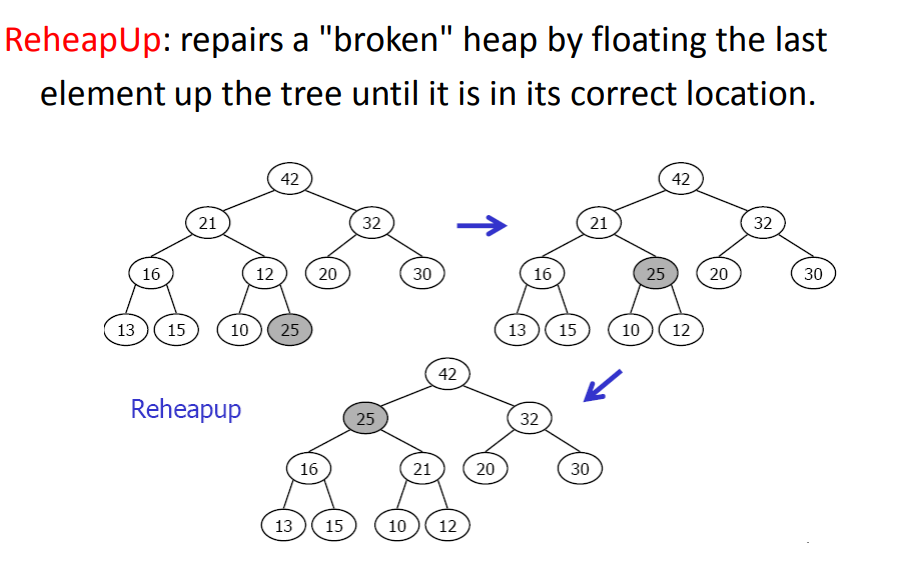
\includegraphics[width=0.8\linewidth]{image2.png}
    \caption{Urca}
    \label{fig:enter-label}
\end{figure}

\subsection*{Coboara/ Percolate/ ReheapDown: }
\begin{figure}[H]
    \centering
    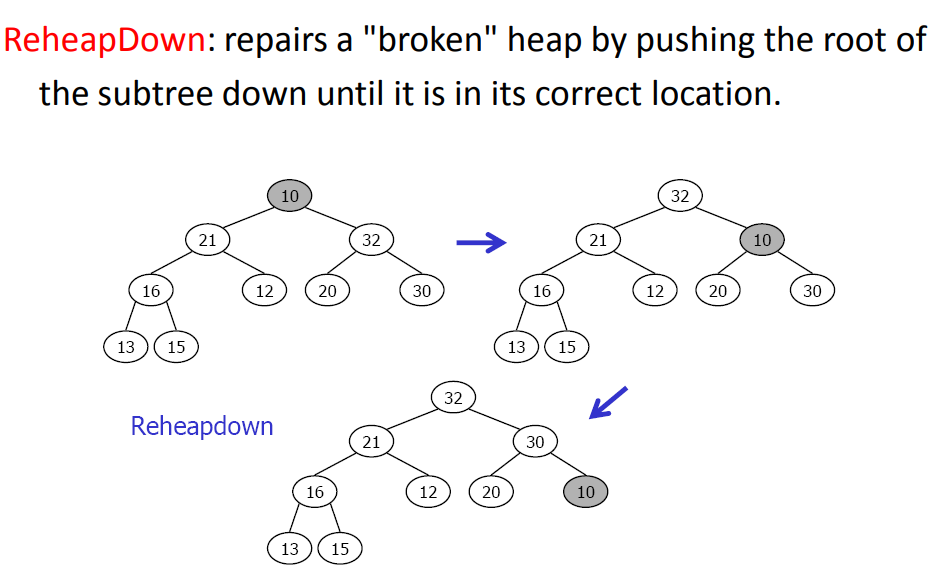
\includegraphics[width=0.8\linewidth]{image.png}
    \caption{Coboara}
    \label{fig:enter-label}
\end{figure}

\subsection*{Insert: }
\begin{figure}[H]
    \centering
    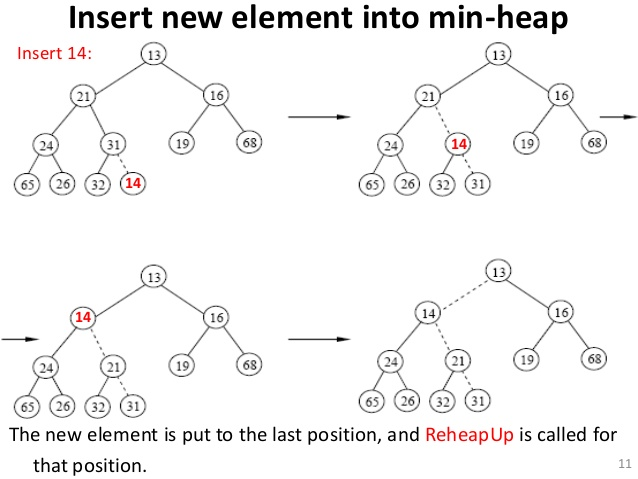
\includegraphics[width=0.8\linewidth]{insert-minheap.png}
    \caption{Insert in min-heap.}
    \label{fig:enter-label}
\end{figure}

\subsection*{Delete: }
\begin{figure}[H]
    \centering
    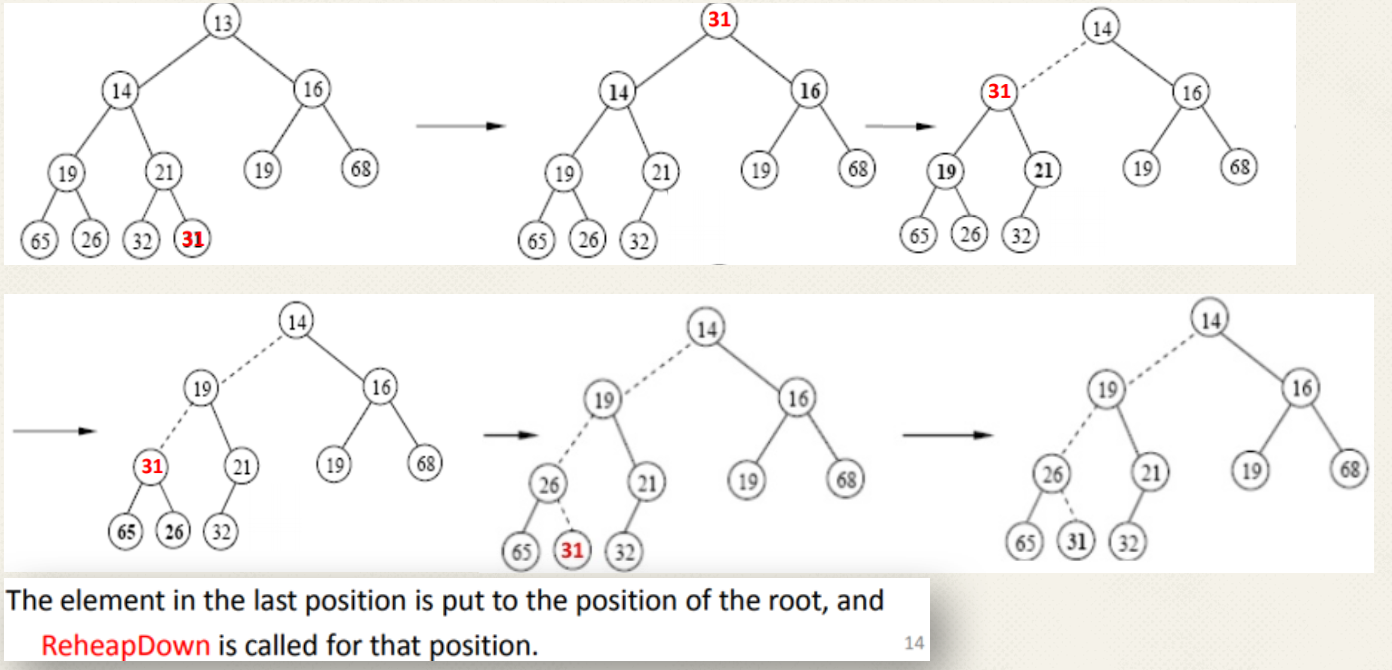
\includegraphics[width=0.85\linewidth]{heap-delete-root.png}
    \caption{Delete root of the heap.}
    \label{fig:enter-label}
\end{figure}

Analog se procedeaza si pentru stergerea oricarui nod din heap. Se interschimba cu ultimul, iar apoi facem \textbf{ReheapDown}.

\subsection*{Heapify}
O alta problema este construirea unui heap. Aceasta poarta numele de \textit{heapify}. Complexitatea este O(n) si nu O(nlog(n)). Punem valorile in heap random. Pentru fiecare nod de la ultimul nivel in sus, facem \textbf{ReheapDown}.

\textbf{Demonstratie complexitate O(n):}

Pentru fiecare coborare vom avea $O(h)$ complexitate. Sunt aprox. $n/2$ frunze in heap. Pentru frunze nu avem ce cobori. Apoi, frunzele au $n/4$ noduri parinte pentru care facem maxim 1 opearatie de swap. Apoi, $n/8$ noduri pentru care facem maxim 2 operatii de swap. Generalizand, obtinem ca numarul de operatii pe care il facem este: 
$$ 
\sum \frac{n}{2^{i}}(i-1) = n \sum\frac{i-1}{2^{i}}
$$

Seria $\sum\frac{i-1}{2^{i}}$ converge la $1$, deci obtinem complexitate O(n).

\subsection*{Combinatorica, Diverse}
\textbf{Numărul minim de elemente dintr-un heap binar de înălțime k}? (Vom presupune că rădăcina heap-ului se află la înălțime 0) este: $2^k$.

\bigskip

\textbf{Se pot gasi elementele maxime / minime intr-un heap de minim / maxim?} Elementele respective se vor afla in frunze, deci trebuie sa parcurgem frunzele heap-ului (aprox. $n/2$ frunze). Asadar, se poate gasi maximul intr-un min-heap sau invers in complexitate O(n).


\subsection*{Merge Heaps}
Deoarece operatia de merge este inceata, exista alte tipuri de heap-uri: \textit{binomiale} si \textit{fibonacci}.

\newpage

\bigskip
\setlength{\tabcolsep}{2pt} 
\begin{tabular}{|l|c|c|c|c|c|}
\hline
 & \textbf{Căutare Min} & \textbf{Ștergere Min} & \textbf{Inserare} & \textbf{Update} & \textbf{Reuniune} \\
\hline
Heap Binar & $\mathcal{O}(1)$ & $\mathcal{O}(\log N)$ & $\mathcal{O}(\log n)$ & $\mathcal{O}(\log n)$ & $\mathcal{O}(n)$ \\
\hline
Heap Binomial & $\mathcal{O}(1)$ & $\mathcal{O}(\log n)$ & $\mathcal{O}(1) \text{ (amortizat)}$ & $\mathcal{O}(\log n)$ & $\mathcal{O}(\log n)$ \\
\hline
Heap Fibonacci & $\mathcal{O}(1)$ & $\mathcal{O}(\log n) \text{ (amortizat)}$ & $\mathcal{O}(1)$ & $\mathcal{O}(1) \text{ (amortizat)}$ & $\mathcal{O}(1)$ \\
\hline
\end{tabular}

\newpage

\subsection{Heapuri Binomiale}
\subsection*{Arbori binomiali}
Un arbore binominal de ordin k:
\begin{itemize}
    \item Are exact $2^{k}$ noduri.
    \item Inaltimea $k$
    \item Sunt exact $C_{i}^{k}$ noduri de inaltime i.
\end{itemize}
\begin{figure}[H]
    \centering
    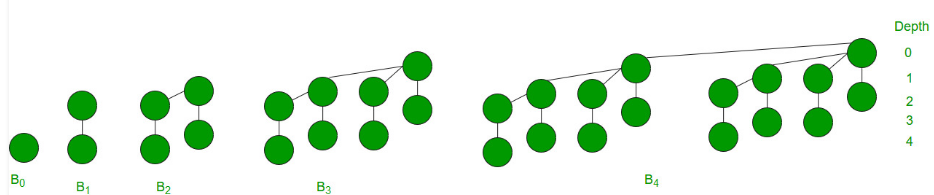
\includegraphics[width=0.85\linewidth]{arbori-binomiali.png}
    \caption{Arbori Binomiali}
    \label{fig:enter-label}
\end{figure}

\subsection{Heapuri Binomiale}
Un heap binomial este o familie de arbori binomiali care au proprietatea de heap minim. Există o singură structură de heap binomial pentru orice mărime.

\begin{figure}[H]
    \centering
    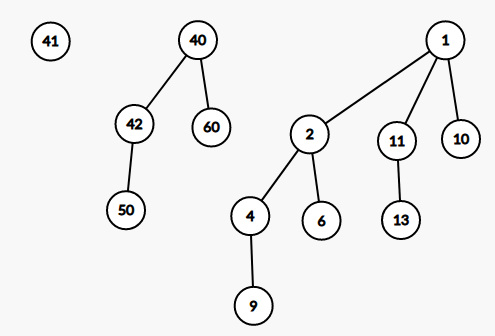
\includegraphics[width=0.6\linewidth]{exemplu-heap-binomial.png}
    \caption{Heap Binomial}
    \label{fig:enter-label}
\end{figure}

Heap-ul din figura este un heap binomial cu 13 noduri($13 = 8 + 4 + 1$).

\textbf{Extragerea minimului}: Vom avea minimul dintre toate radacinile arborilor binomiali (O(log(n)) complexitate) sau retinem minimul si il updatam la fiecare alta operatie (O(1) complexitate).

\textbf{Merge}: Se face astfel: Parcurgem cele doua heap-uri binomiale si combinam arborii binomiali de acelasi rang. Cand obitnem un arbore binomial il putem folosi in reuniune cu alti arbori. Este ca o suma pe biti si pozitile bitilor setati din suma vor fi arborii binomiali pe care ii obtinem.Complexitate: O(log(m+n)).

\textbf{Insert}: vom crea un arbore binomial de rang 1 cu un singur nod si vom da merge cu heap-ul initial. Complexitate: O(log(n)) (vine din merge).

\textbf{Stergere minim}: Cand stergem, eliminam minimul, iar apoi facm reuniune. Complexitate: O(log(n)) (vine din merge).

\subsection{Heapuri Fibonnaci}

\begin{itemize}
    \item Heapurile Fibonacci sunt o colecție de arbori care au proprietatea de ordonare de heap (arborii nu trebuie să fie binomiali). \textbf{Putem avea si arbori de aceeasi dimesniune in heap.}
    \item Arborii dintr-un heap Fibonacci nu sunt ordonați.
    \item Arborii din componență au mărimi \textbf{puteri ale lui 2}. Fiii vor fi arbori de mărime $1,…, k-1$, dar nu neapărat sortați de la stânga la dreapta.
\end{itemize}

\begin{figure}[H]
    \centering
    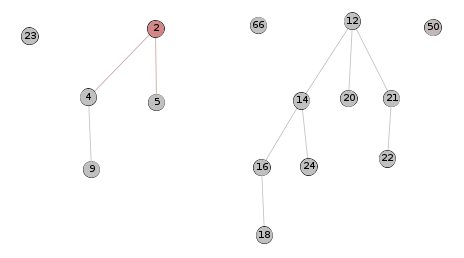
\includegraphics[width=0.75\linewidth]{fibonacci-heap.png}
    \caption{Fibonacci Heap}
    \label{fig:enter-label}
\end{figure}

Structura unui heap fibonacci:
\begin{itemize}
    \item Listă dublu înlănțuită între rădăcini
    \item Link către un fiu
    \item Listă dublu înlănțuită între frați
    \item Link către tată
\end{itemize}

\begin{figure}[H]
    \centering
    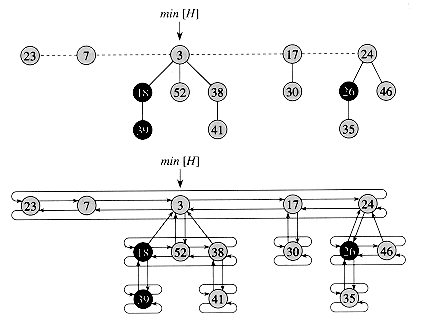
\includegraphics[width=0.75\linewidth]{fibonacci-heap2.png}
    \caption{Fibonacci Heap Implementation}
    \label{fig:enter-label}
\end{figure}

\textbf{Extragere minim}: retinem un pointer catre minim care il actualizam la fiecare operatie. Complexitate: O(1).

\textbf{Inserare}: cream un nou arbore cu un singur element si il atasam heap-ului. Nu facem reuniune. Complexitate: O(1)

\textbf{Merge}: concatenam lista de radacini ale primului heap la cel de-al doilea. Modificam pointer-ul catre minim. Complexitate: O(1).

\textbf{Stergere minim}: Stergem minimul si ramanem cu doi arbori liberi (subarborii nodului sters). La extragerea minimului vom consolida heap-ul, adica se face reuniune similar cu heap-urile binomiale. \textbf{Consolidarea heap-ului}: Se calculeaza gradul unui arbore, ca fiind inaltimea arborelui si arborii cu acelasi grad se reunesc. 

\subsection{Arbori Huffman}
Codurile Huffman reprezintă o tehnică eficientă pentru compactarea datelor. Scopul este ca, pentru fiecare caracter, să alegem o metodă optimă pentru a o scrie în binar.

\textbf{Constructia unui arbore Huffman}
Luam frecventele caracterelor in ordine crescatoare. Unim de fiecare data cele mai mici 2 valori. Frecventa noului nod obtinut o bagam in lista si repetem procesul.

\textbf{Observatie: Arborii Huffman nu sunt unici!}

\begin{figure}[H]
    \centering
    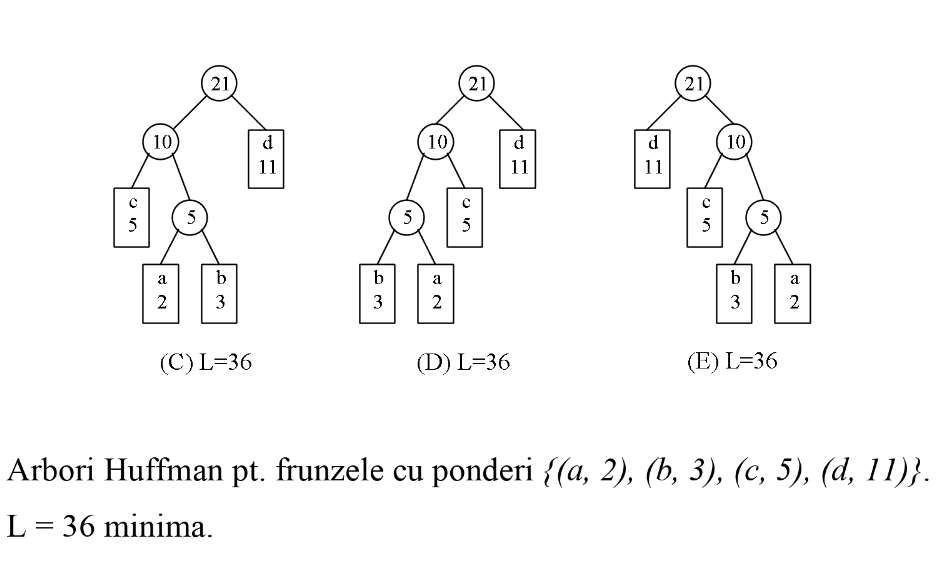
\includegraphics[width=0.75\linewidth]{huffman.png}
    \caption{Arbori Huffman Exemplu}
    \label{fig:enter-label}
\end{figure}

\section{Arbori binari de cautare echilibrati}

Cautam modalitati de a mentine adancimea unui arbore cat mai apropiata de log(n).

\textbf{Teorema 13.6.} Înălţimea medie a unui arbore binar de căutare construit aleator cu n chei distincte este O(lg n).

\subsection{Red Black Trees}
\begin{itemize}
    \item Fiecare nod e fie roșu, fie negru
    \item Rădăcina e mereu neagră
    \item Nu putem avea două noduri adiacente roșii
    \item Orice drum de la un nod la un descendent NULL are același număr de noduri negre
\end{itemize}

\subsection{AVL Trees}
Pentru AVL-uri definim \textbf{factorul de echilibru} al unui nod: $BF(X) = h(subarbDrp(X)) - h(subarbStg(X))$, unde h este inaltimea unui arbore.

Un arbore AVL este un arbore care are $BF(x) <= 1$, pentru orice nod $x$.

Pentru rebalansarea arborelui se aplica rotatii: rotație stânga-stânga, rotație stânga-dreapta, rotație dreapta-stânga, rotație dreapta-dreapta.

\section{Skip Lists}
Sunt structuri de date echilibrate care ajuta la cautare rapida. Elementele \textbf{sunt sortate}.

Structura:
\begin{itemize}
    \item Skip-listul este o lista inlatuita, dar extinsa pe mai multe nivele.
    \item La fiecare nivel adăugat, sărim peste o serie de elemente față de nivelul anterior
    \item Nivelele au legături între ele
\end{itemize}

\begin{figure}[H]
    \centering
    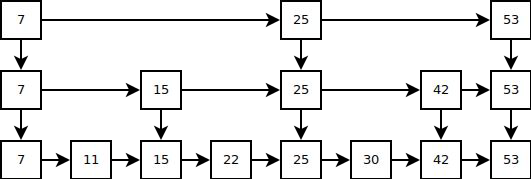
\includegraphics[width=0.75\linewidth]{skip-lists.png}
    \caption{Skip List}
    \label{fig:enter-label}
\end{figure}

\subsection*{Cautare}

\begin{itemize}
    \item Începem căutarea cu primul nivel (cel mai de sus) 2)
    \item Avansăm în dreapta, până când, dacă am mai avansa, am merge prea departe (adică elementul următor este prea mare)
    \item Ne mutăm în următoarea listă (mergem în jos)
    \item Reluăm algoritmul de la pasul 2)
    
\end{itemize}

\begin{figure}[H]
    \centering
    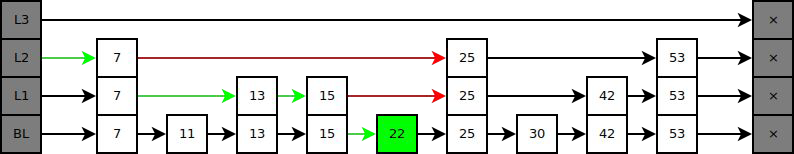
\includegraphics[width=0.75\linewidth]{skip-list-ex1.png}
    \caption{Cautare elementul 22}
    \label{fig:enter-label}
\end{figure}

\subsection*{Inserare}
\begin{itemize}
    \item Vrem să inserăm elementul x. Observație: Lista de jos trebuie să conțină toate elementele, deci căutăm locul lui x în lista de jos → search(x) si adaugam x in locul respectiv.
    \item Cum alegem în ce altă listă să fie adăugat?Alegem metoda probabilistică:
    
    \begin{itemize}
        \item aruncăm o monedă
        \item  dacă pică Stema - o adăugăm în lista următoare și aruncăm din nou moneda
        \item dacă pică Banul - ne oprim
    \end{itemize}
\end{itemize}

În medie vom aveae $\frac{1}{2}$ elemente nepromovate, $\frac{1}{4}$ elemente promovate 1 nivel, $\frac{1}{8}$ elemente promovate 2 nivele si tot asa.

Deci, obtinem o complexitate O(log(n))

\subsection*{Stergere}
Stergem elementul x din toate listele in care se afla. Complexitate: O(log(n)).

\section{Treap}
Structură de date arborescentă care menține simultan proprietatea de arbore binar de căutare (BST) și cea de max-heap. 

Puțin mai formal, fie $(X_{i}, Y_{i})$ nodurile arborelui. Treap-ul asigură structură de ABC pentru toți $X_i$, iar în $Y_i$, structura de max-heap.

\begin{figure}[H]
    \centering
    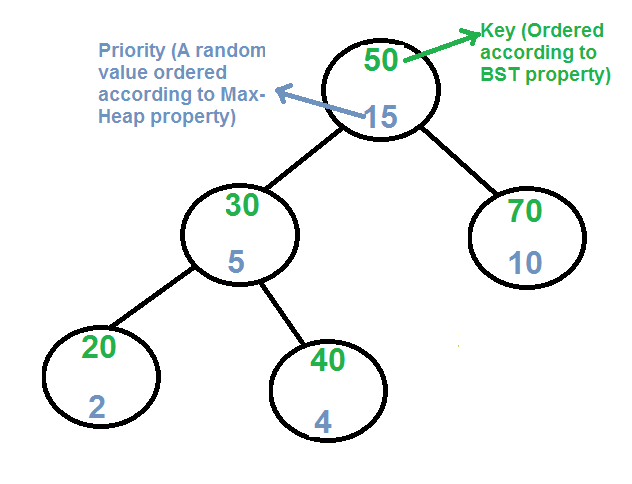
\includegraphics[width=0.5\linewidth]{treap1.png}
    \caption{Treap}
    \label{fig:enter-label}
\end{figure}

De ce treapuri? Sunt usor de implementat. Cu puține modificări, permit abordarea multor tipuri de query-uri și update-uri (sume, cmmdc, rotații etc pe intervale).

\begin{figure}[H]
    \centering
    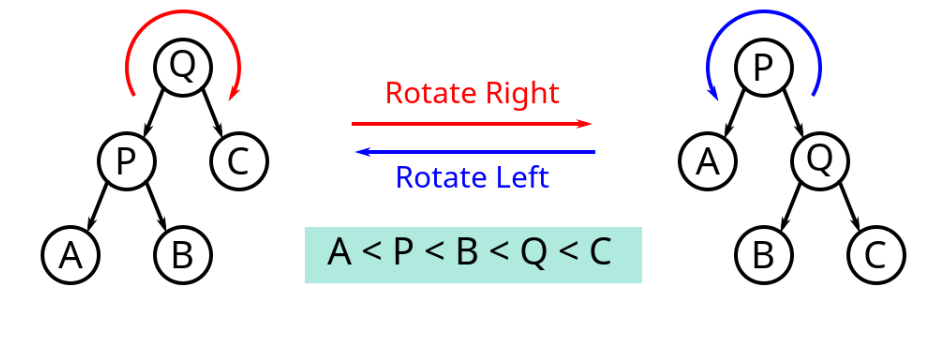
\includegraphics[width=0.5\linewidth]{rotatii1.png}
    \caption{Rotatii pe arbori}
    \label{fig:enter-label}
\end{figure}

\subsection*{Inserare}
La inserare, inseram exact ca intr-un BST obisnuit, iar dupa, pe recursie, rotim în sens invers subarborele cu rădăcina în nodul curent, în funcție de tipul fiului (stâng/drept).

\subsection*{Cautare}
Exact ca la un BST obisnuit.

\subsection*{Stergere}
Există trei cazuri în care se poate afla un nod pe care vrem să-l ștergem:

\begin{itemize}
    \item E frunză -> Îl ștergem direct.
    \item Are numai un fiu -> Fiul ia locul nodului respectiv
    \item Are doi fii -> Rotim în locul rădăcinii subarborelui făcut din nodul curent fiul cu prioritatea cea mai mare. Repetăm algoritmul până când ne aflăm în unul dintre primele două cazuri. 
\end{itemize}


\section{Range Minimum Query}
Se dă un vector. Răspundeți cât mai eficient la întrebări de genul: Care este cel mai mic element din intervalul $(i, j)$?

\begin{table}[h!]
\centering
\label{tab:ds_comparison}
\begin{tabular}{lcccc}
    \toprule
    \textbf{Operation} & \textbf{Segment Tree} & \textbf{RMQ} & \textbf{Batog(sqrt)} \\
    \midrule
    \textbf{Build} & $\mathcal{O}(n)$ & $\mathcal{O}(n \log n)$ & $\mathcal{O}(n)$ \\
    \textbf{Query} & $\mathcal{O}(\log n)$ & $\mathcal{O}(1)$ & $\mathcal{O}(\sqrt{n})$  \\
    \textbf{Point Update} & $\mathcal{O}(\log n)$ & N/A (not supported) & $\mathcal{O}(1)$ \\
    \bottomrule
\end{tabular}
\caption{Comparison of Segment Tree, Sparse Table (RMQ) Complexities and Sqrt Decomposition(Batog)}
\end{table}

\textbf{Atentie}: RMQ se preteaza pentru situatia in care nu avem update-uri. Altfel, daca exista update-uri, folosim un arbore de intervale sau batog.

Exemplu:

\bigskip
\begin{tabular}{|c|c|c|c|c|c|c|c|c|c|c|}
\hline
0 & 1 & 2 & 3 & 4 & 5 & 6 & 7 & 8 & 9 & 10\\
\hline
4 & 2 & 7 & 8 & 3 & 5 & 9 & 1 & 6 & 2 & 9 \\
\hline
\end{tabular}
\bigskip

Minimul pe (0,3) este 2. Minimul pe (5,9) este 2.

Pentru fiecare poziție i din v, vom calcula mai multe minime. Pentru fiecarte secvență de lungime putere de 2 care începe la poziția i, vom calcula minimul dintre elementele ei.

Deci, pentru fiecare poziție din v vom avea maxim log(n) minime de calculat (atâtea puteri de 2 sunt mai mici sau egale decât n).

\textbf{Astfel, vom obține o matrice r[p][i] = minimul din v pentru elementele dintr-o secvență de lungime $2^p$ care începe la poziția i.}

\bigskip
\begin{tabular}{|l|c|c|c|c|c|c|c|c|c|c|c|}
\hline
v: & 4 & 2 & 7 & 8 & 3 & 5 & 9 & 1 & 6 & 2 & 9 \\
\hline
r: & & & & & & & & & & & \\
\hline
$2^0$ & 4 & 2 & 7 & 8 & 3 & 5 & 9 & 1 & 6 & 2 & 9 \\
\hline
$2^1$ & 2 & 2 & 7 & 3 & 3 & 5 & 1 & 1 & 6 & 2 & 9 \\
\hline
$2^2$ & 2 & 2 & 3 & 3 & 1 & 1 & 1 & 1 & 2 & 2 & 9 \\
\hline
$2^3$ & 1 & 1 & 1 & 1 & 1 & 1 & 1 & 1 & 2 & 2 & 9 \\
\hline
\end{tabular}
\bigskip

\subsection*{Constructie}
Un element de pe linia p se calculează ca minimul a două elemente de pe linia $p-1$:
$$r[p][i] = min (r[p-1][i], r[p-1][i+2
p-1]).$$

Având deja linia 0 cunoscută nu ne rămâne decât să calculăm valorile linie cu linie, în ordinea crescătoare a indicilor de linii.

\subsection*{Query}
La fiecare interogare primim capetele unui interval, $[st, dr]$ care, evident, nu este neapărat de lungime putere de 2.

Pentru a raspunde la query putem face o descompunere in baza 2 si obtinem O(log(n)). Dar, putem sa facem in O(1).
Pentru acest lucru, să considerăm cea mai mare putere de 2 mai mică sau egală decât L (notăm cu len această valoare). 

Acum să considerăm, intervalul de lungime len care începe la poziția st și pe cel de lungime len care se termină la poziția dr. 

Aceste doua intervale acopera complet intervalul nostru, deci putem face minimul / maximul lor si acesta este raspunsul la query.

\begin{figure}[H]
    \centering
    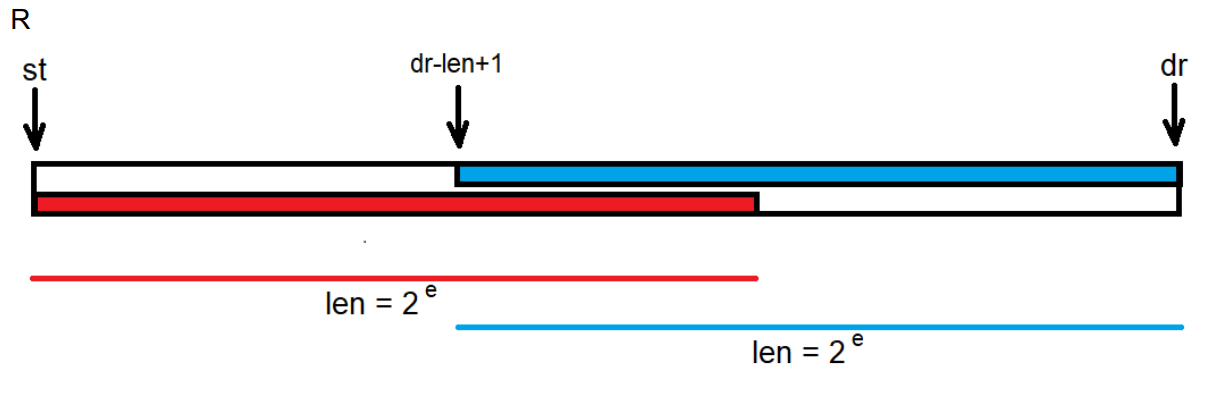
\includegraphics[width=0.75\linewidth]{rmq.png}
    \caption{RMQ Query}
    \label{fig:enter-label}
\end{figure}

\subsection{Lowest Ancestor (LA)}
Se dă un arbore. Răspundeți cât mai eficient la întrebări de genul: Se dă un nod și un întreg k. Care este strămoșul de nivel k al nodului dat?

\begin{figure}[H]
    \centering
    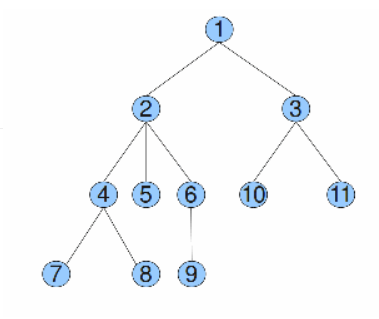
\includegraphics[width=0.45\linewidth]{lca-tree.png}
    \caption{Tree Example}
    \label{fig:enter-label}
\end{figure}

$$LA(2,1) = 1, LA(9,1) = 6, LA(9,2) = 2, LA(6,4) = -1$$

Mai multe rezolvari posibile:
\begin{itemize}
    \item Parcurg din tata in tata. Complexitate: $O(n)$ pe query si $O(1)$ memorie.
    \item Retin un map unde stiu toti stramosii nodurilor. Preprocesare si memorie: $O(n \cdot h)$ si $O(1)$ pe query.
    \item Sqrt Decomposition (Batog). Țin pointer catre tatăl de ordin radical din n. Obtinem $O(n)$ memorie suplimentara si $O(\sqrt{n})$ pe query.

    \item \textbf{Binary Lifting:} Pentru fiecare nod, țin tații de înălțime $1, 2, 4, 8, 16, …$. La query facem similar cu cautarea binara. Sarim cu cea mai mare putere de 2 posibila.Complexitate $O(n \cdot log(n))$ preprocesoare, $O(n\cdot log(n))$ memorie suplimentară si $O(log(n))$ pe query.
\end{itemize}

\subsection{Lowest Common Ancestor (LCA)}
Răspundeți cât mai eficient la întrebări de genul: Se dau două noduri într-un arbore. Găsiți cel mai apropiat strămoș comun.

\begin{figure}[H]
    \centering
    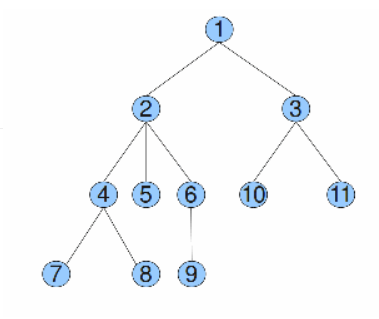
\includegraphics[width=0.45\linewidth]{lca-tree.png}
    \caption{Tree Example}
    \label{fig:enter-label}
\end{figure}

$$LCA(4,9) = 2, LCA(4,11) = 1, LCA(7,6) = 2$$

Una dintre aplicatiile \textbf{structurii RMQ} este determinarea LCA-ului.


\begin{itemize}
    \item \textbf{Liniarizam arobrele printr-o parcurgere Euler}: Începem o parcurgere RSD din rădăcină și scriem fiecare nod de fiecare dată când trecem prin el.
    \item Pentru fiecare nod, reținem și distanța de la el la rădăcină.
    \item Pentru fiecare nod, reținem și prima sa apariție în parcurgerea Euler.
    \item $LCA(i,j) = RMQ(first[i], first[j])$. Unde RMQ calculeaza minimul pe vectorul de distante pana la radacina.
    \item Acum putem raspunde la query-uri $LCA(x,y)$ in $O(1)$.
\end{itemize}

\textbf{Complexitate:  $O(nlog(n) + q)$}

\begin{figure}[H]
    \centering
    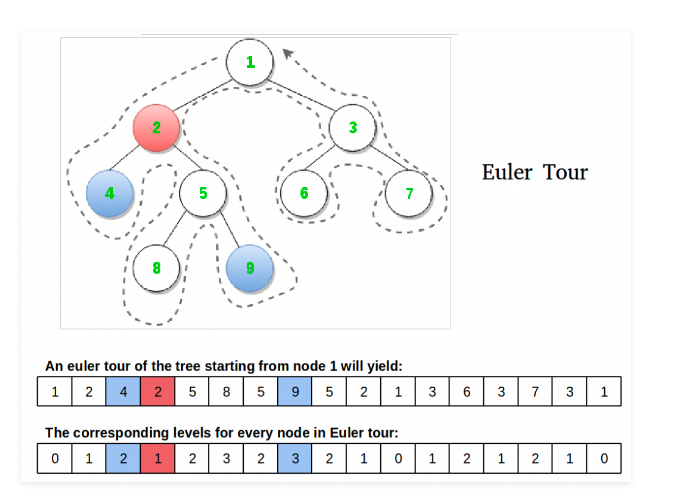
\includegraphics[width=0.75\linewidth]{lca-euler-tour.png}
    \caption{Euler Tour}
    \label{fig:enter-label}
\end{figure}

\section{Trie (Prefix Tree)}
\textbf{Problema:} Am mai multe cuvinte pe care le tin minte și apoi am întrebări de genul: este cuvântul dat în acea listă sau nu? Solutii posibile:
\begin{itemize}
    \item Hash-uri, $O(l)$ (unde l e lungimea cuvântului) pe query si $O(n \cdot l)$ memorie.
\end{itemize}

\textbf{Problema: }
Am mai multe cuvinte și apoi am întrebări de genul:
Este cuvântul în dicționar sau nu? Care este cel mai lung prefix al cuvântului în dicționar? Solutii posibile:

\begin{itemize}
    \item Nu mai merge cu hash-uri.
    \item Sortăm toate cuvintele lexicografic și apoi căutăm binar. \textbf{$O(n \cdot l)$ memorie și $O(log(n) \cdot l)$}
    \item Ținem toate cuvintele într-un arbore binar de căutare echilibrat. \textbf{$O(n \cdot l)$ memorie și $O(log(n) \cdot l)$}
\end{itemize}

Implementare Trie:
\begin{itemize}
    \item Fiecare nod are un vector cu 26 de vecini, una pentru fiecare literă (sau mărimea alfabetului).
    \item Ce facem dacă alfabetul e mare? Fiecare nod ține un hash-map care, pentru fiecare literă, ține pointer-ul către nodul cu acea literă.
\end{itemize}

\begin{figure}[H]
    \centering
    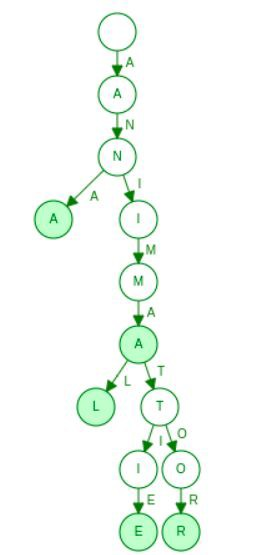
\includegraphics[width=0.3\linewidth]{trie.png}
    \caption{Trie cu cuvintele ana, animator, animație, animal, anima.}
    \label{fig:enter-label}
\end{figure}

\subsection*{Inserare}
Pornim din rădăcină și, la fiecare literă, mergem în nodul corespunzător literei. Eventual creăm acel nod. \textbf{Complexitate: $O(l)$}

\begin{figure}[H]
    \centering
    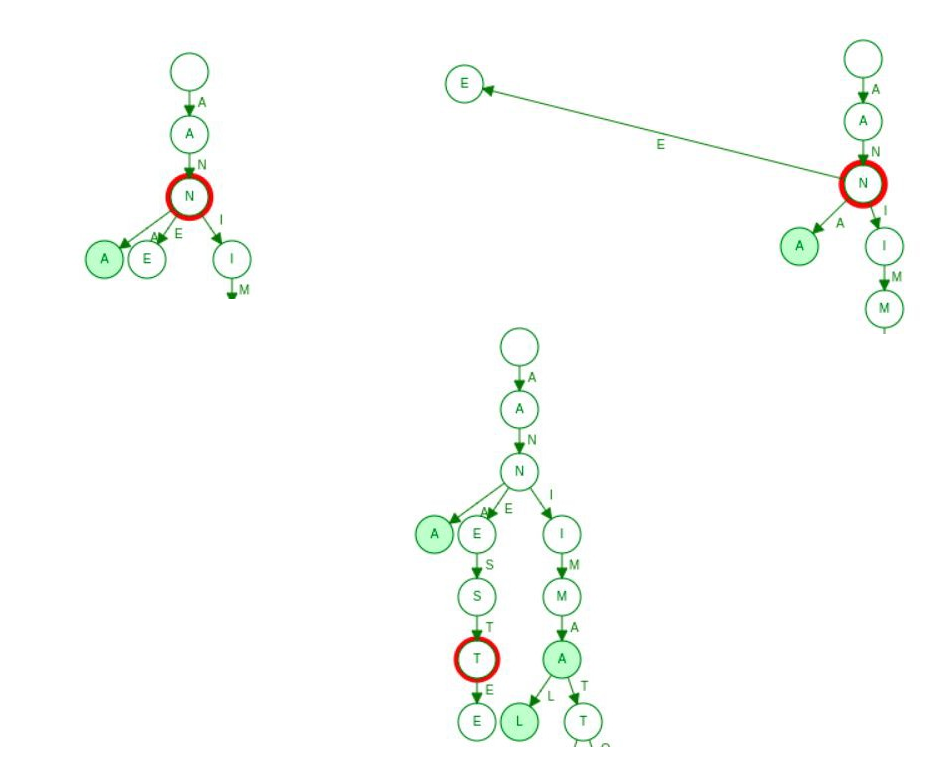
\includegraphics[width=0.75\linewidth]{insert-trie.png}
    \caption{Inserare in trie}
    \label{fig:enter-label}
\end{figure}

\subsection*{Cautare}

Cautarea unui cuvant din dictionar: 
\begin{itemize}
    \item Pornim din rădăcină și mergem, la fiecare pas, pe litera corespunzătoare.
    \item Complexitate $O(l)$ pentru căutare reușită.
    În practică, mai rapid pentru căutare nereușită.
\end{itemize}

Căutare prefix maxim: Căutăm elementul până nu găsim nod corespunzător acelei litere. \textbf{Complexitate $O(l)$.}

\subsection*{Sortarea lexicografica in trie}
Odată ce trie-ul este construit, sortarea în ordine lexicografică poate fi realizată printr-un traversare în preordine (preorder traversal). Într-un trie, o traversare în preordine va vizita nodurile în ordine lexicografică, deoarece:

\begin{itemize}
    \item Nodurile sunt vizitate de la rădăcină spre frunze.
    \item La fiecare nivel, vizităm nodurile în ordinea alfabetică a literelor.
\end{itemize}

\end{document}




